\documentclass[12pt,a4paper]{report}

\usepackage[utf8]{inputenc} % pentru suport diacritice
\usepackage[romanian]{babel} % setări pentru limba română 
\renewcommand\familydefault{\sfdefault} % sans serif

\usepackage[margin=2.54cm]{geometry}	% dimensiuni pagină și margini
\usepackage{graphicx} % support the \includegraphics command and options

% formatting sections and subsections
\usepackage{textcase}
\usepackage[titletoc, title]{appendix}
\usepackage{titlesec}
\titleformat{\chapter}{\large\bfseries\MakeUppercase}{\thechapter}{2ex}{}[\vspace*{-1.5cm}]
\titleformat*{\section}{\large\bfseries}
\titleformat*{\subsection}{\large\bfseries}
\titleformat*{\subsubsection}{\large\bfseries}

\usepackage{chngcntr}
\counterwithout{figure}{chapter} % no chapter number in figure labels
\counterwithout{table}{chapter} % no chapter number in table labels
\counterwithout{equation}{chapter} % no chapter number in equation labels

\usepackage{booktabs} % for much better looking tables
\usepackage{url} % Useful for inserting web links nicely
\usepackage[bookmarks,unicode,hidelinks,breaklinks]{hyperref}
\usepackage{breakurl}
\def\UrlBreaks{\do\/\do-}

\usepackage{array} % for better arrays (eg matrices) in maths
\usepackage{paralist} % very flexible & customisable lists (eg. enumerate/itemize, etc.)
\usepackage{verbatim} % adds environment for commenting out blocks of text & for better verbatim
\usepackage{subfig} % make it possible to include more than one captioned figure/table in a single float
\usepackage{enumitem}
\setlist{noitemsep}

%%% HEADERS & FOOTERS
\usepackage{fancyhdr}
\pagestyle{empty}
\renewcommand{\headrulewidth}{0pt}
\renewcommand{\footrulewidth}{0pt}
\lhead{}\chead{}\rhead{}
\lfoot{}\cfoot{\thepage}\rfoot{}



\newcommand{\HeaderLineSpace}{-0.25cm}
\newcommand{\UniTextRO}{UNIVERSITATEA POLITEHNICA DIN BUCUREȘTI \\[\HeaderLineSpace] 
FACULTATEA DE AUTOMATICĂ ȘI CALCULATOARE \\[\HeaderLineSpace]
DEPARTAMENTUL DE CALCULATOARE\\}
\newcommand{\DiplomaRO}{PROIECT DE DIPLOMĂ}
\newcommand{\AdvisorRO}{Coordonator științific:}
\newcommand{\BucRO}{BUCUREȘTI}

\newcommand{\UniTextEN}{UNIVERSITY POLITEHNICA OF BUCHAREST \\[\HeaderLineSpace]
FACULTY OF AUTOMATIC CONTROL AND COMPUTERS \\[\HeaderLineSpace]
COMPUTER SCIENCE AND ENGINEERING DEPARTMENT\\}
\newcommand{\DiplomaEN}{DIPLOMA PROJECT}
\newcommand{\AdvisorEN}{Thesis advisor:}
\newcommand{\BucEN}{BUCHAREST}

\newcommand{\frontPage}[6]{
\begin{titlepage}
\begin{center}
{\Large #1}  % header (university, faculty, department)
\vspace{50pt}
\begin{tabular}{p{6cm}p{4cm}}

\includegraphics[scale=0.8]{pics/upb-logo.jpg} &
	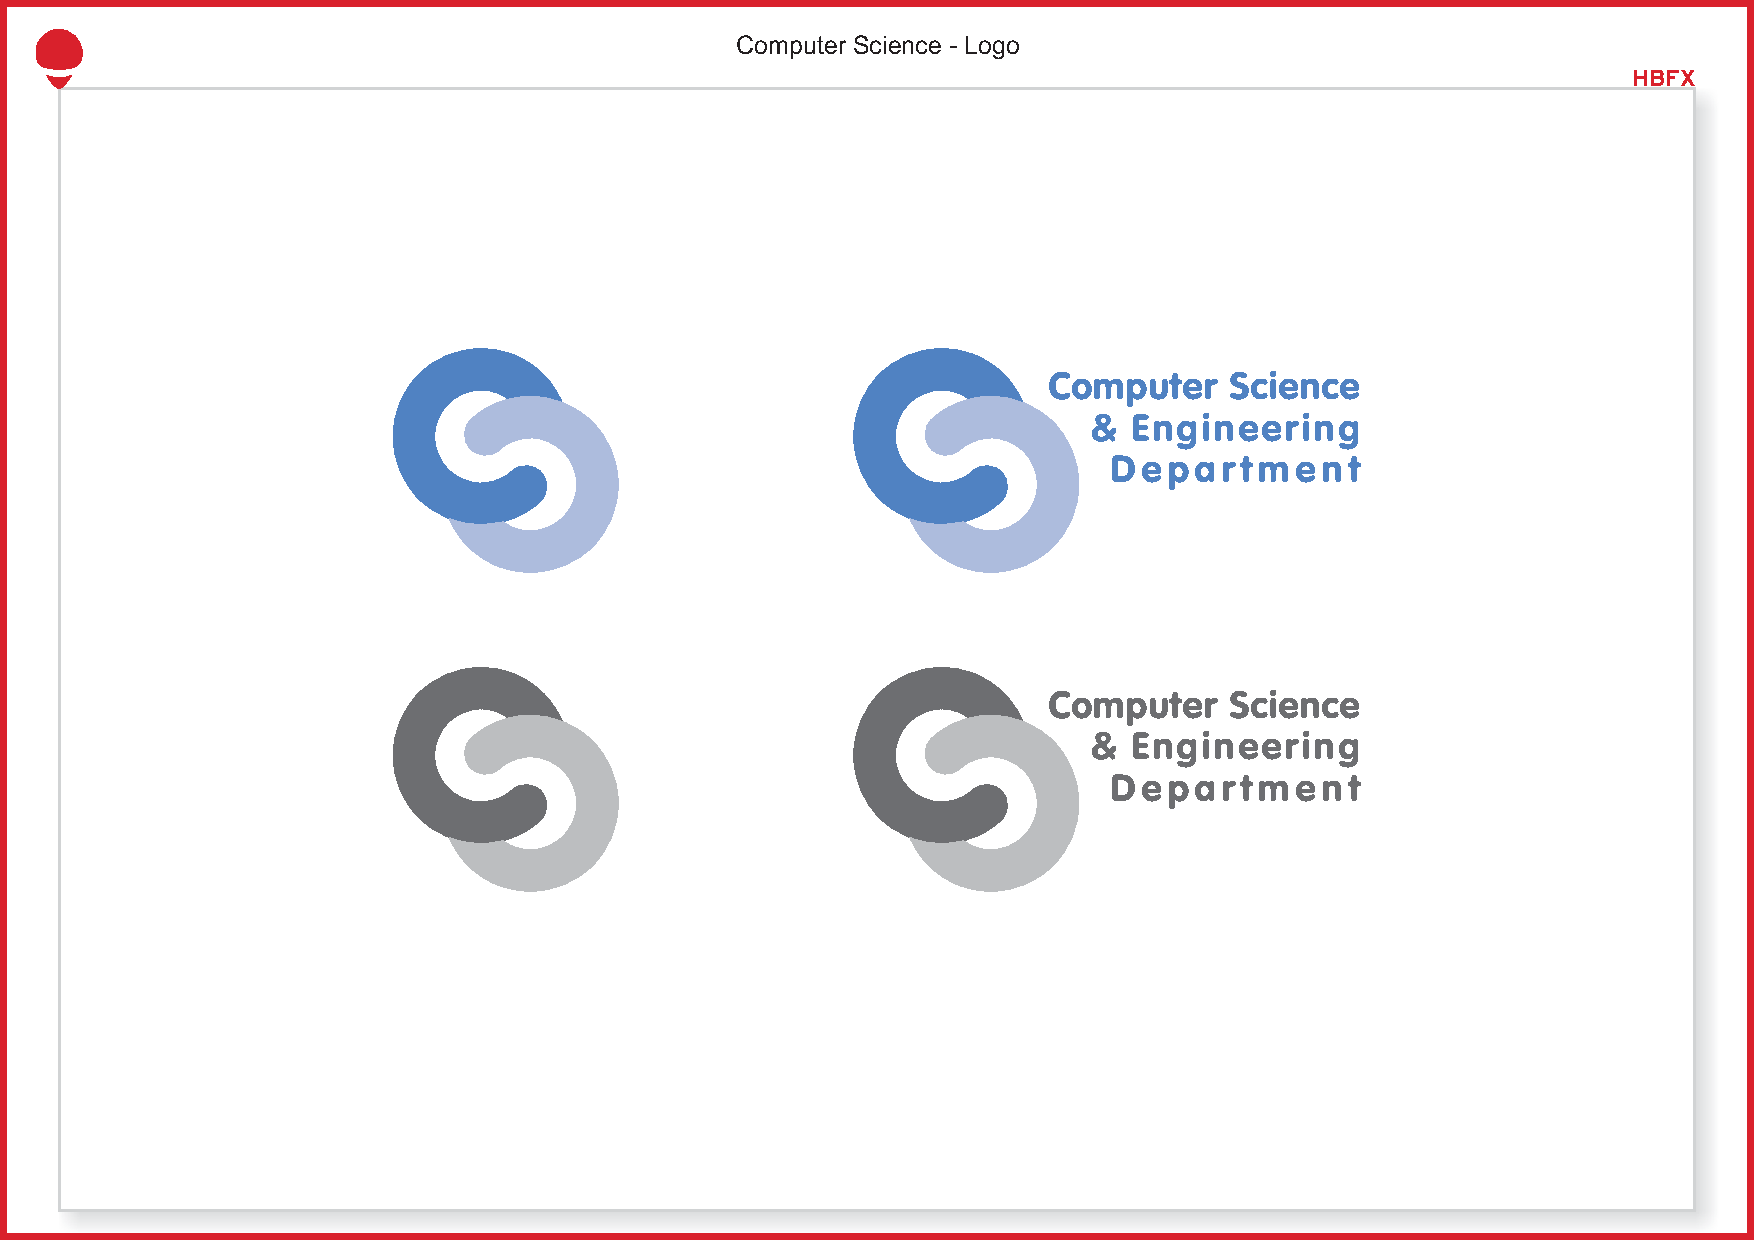
\includegraphics[scale=0.5,trim={14cm 11cm 2cm 5cm},clip=true]{pics/cs-logo.pdf}
\end{tabular}

\vspace{105pt}
{\Huge #2}\\                           % diploma project text
\vspace{40pt}
{\Large #3}\\ \vspace{0pt}  % project title
{\Large #4}\\                          % project subtitle
\vspace{40pt}
{\LARGE \Name}\\                   % student name
\end{center}
\vspace{60pt}
\begin{tabular*}{\textwidth}{@{\extracolsep{\fill}}p{6cm}r}
&{\large\textbf{#5}}\vspace{10pt}\\      % scientific advisor
&{\large \Advisor}                                    % advisor name
\end{tabular*}
\vspace{20pt}
\begin{center}
{\large\textbf{#6}}\\                                % bucharest
\vspace{0pt}
{\normalsize \Year}
\end{center}
\end{titlepage}
}

\newcommand{\frontPageRO}{\frontPage{\UniTextRO}{\DiplomaRO}{\ProjectTitleRO}{\ProjectSubtitleRO}{\AdvisorRO}{\BucRO}}
\newcommand{\frontPageEN}{\frontPage{\UniTextEN}{\DiplomaEN}{\ProjectTitleEN}{\ProjectSubtitleEN}{\AdvisorEN}{\BucEN}}

\linespread{1.5}
\setlength\parindent{0pt}
\setlength\parskip{.28cm}

%% Abstract macro
\newcommand{\AbstractPage}{
\begin{titlepage}
\textbf{\large SINOPSIS}\par
\AbstractRO\par\vfill
\textbf{\large ABSTRACT}\par
\AbstractEN \vfill
\end{titlepage}
}

%% Thank you macro
\newcommand{\ThanksPage}{
\begin{titlepage}
{\noindent \large\textbf{MULȚUMIRI}}\\
\Thanks
\end{titlepage}
}



%%%%%%%%%%%%%%%%%%%%%%%%%%%%%%%%%%%%%%%%%%%%%%%%%%   
%%
%%          End of template definitions
%%   
%%%%%%%%%%%%%%%%%%%%%%%%%%%%%%%%%%%%%%%%%%%%%%%%%%


%%% Puteți elimina aceste linii din lucrare, servesc numai pentru template.
\newcommand{\worktype}[1]{[\textit{#1}] }
\newcommand{\dezvoltare}{\worktype{Dezvoltare de produs}}
\newcommand{\cercetare}{\worktype{Cercetare}}
\newcommand{\ambele}{\worktype{Ambele}}
%%%


%%
%%   Campurile de mai jos trebuie modificate de autor. Modificati doar continutul, nu si numele fiecarei definitii
%%
\newcommand{\ProjectTitleRO}{Analiza de date de trafic de rețea pentru offloading mobil}
%\newcommand{\ProjectSubtitleRO}{Subtitlu (ex: versiunea 2018)}
\newcommand{\ProjectTitleEN}{Network traffic data analysis for mobile offloading}
%\newcommand{\ProjectSubtitleEN}{Subtitle (eg: 2018 version)}
\newcommand{\Name}{Teodora-Ioana Brehuescu}
\newcommand{\Advisor}{Șl.dr.ing. Radu-Ioan Ciobanu}
\newcommand{\Year}{2020}

% Setări document
\title{Proiect de diplomă}
\author{\Name}
\date{\Year}

%%
%%   Campurile aferente rezumatului
%%
\newcommand{\AbstractRO}{Popularitatea de care se bucură smartphone-urile, dar și dispozitivele IoT, au dus la creșterea volumului de trafic pe care trebuie să îl gestioneze operatorii de rețea. Întrucât modificările la nivelul infrastructurii telecom sunt costisitoare, atenția se mută asupra metodelor de offloading care pot fi aplicate la nivelul utilizatorilor. În acest raport vor fi prezentate soluțiile existente de analiză a traficului precum și modul de funcționare al acestora, pentru a motiva alegerea unei anumite interfețe.}

\newcommand{\AbstractEN}{The popularity of smartphones and IoT devices caused a growth in the amount of traffic that must be 
managed by network operators. Considering how expensive it is to change the telecom infrastructure, shifting to offloading techniques applied at the user level could be an alternative.The aim of this paper is to present existing solutions of traffic analysis so that the appropriate interface would be chosen.}

\begin{document}

\frontPageRO
\frontPageEN

\begingroup
\linespread{1}
\tableofcontents
\endgroup

\AbstractPage

\chapter{Introducere}\pagestyle{fancy}
Numărul dispozitivelor mobile și a celor din IoT este într-o continuă creștere, iar acest lucru necesită o infrastructură de rețea cât mai complexă care să suporte volumul de trafic generat de acestea. Întrucât modificările la nivelul operatorilor de rețea sunt mult mai costisitoare, o variantă mai fezabilă ar consta în prioritizarea traficului la nivelul interfețelor pe care le dețin dispozitivele. Altfel spus, într-o zonă aglomerată, precum un stadion sau locația unui concert, congestia de la nivelul celulelor de comunicație ar putea fi evitată prin conectarea utilizatorilor la Wi-Fi. În acest caz, conectarea la Wi-Fi ar fi soluția cea mai bună, dar limitări legate de zona de acoperire sau pierderea de pachete pot să constituie dezavantaje majore în alte situații. Luarea unor astfel de decizii se poate face prin analizarea de date de trafic, stabilirea și măsurarea unor metrici relevante în aplicarea algoritmilor de offloading pentru a alege interfața cea mai optimă pe care să fie transmis traficul.

În prima \textbf{parte a lucrării de cercetare} va fi prezentată motivația care să la baza necesității de analizare a traficului în vederea selectării unei anumite interfețe. Tot în acest raport vor fi prezentate soluțiile existente, aplicații care folosesc metode de offloading precum și modul de funcționarea a acestora.

\section{Context}
Conform Statista~\cite{statisca_Iot_forecast} până în anul 2025, la nivel mondial, se vor înregistra aproximativ 75.44 miliarde de dispozitive IoT. După cum se poate observa în Figura \ref{fig:IoT_forescat}, în ultimii 5 ani, numărul acestora s-a dublat și prezintă o tendință de creștere de până la 5 ori mai mare față de numărul înregistrat în anul 2015. 

\begin{figure}[th]
\centering
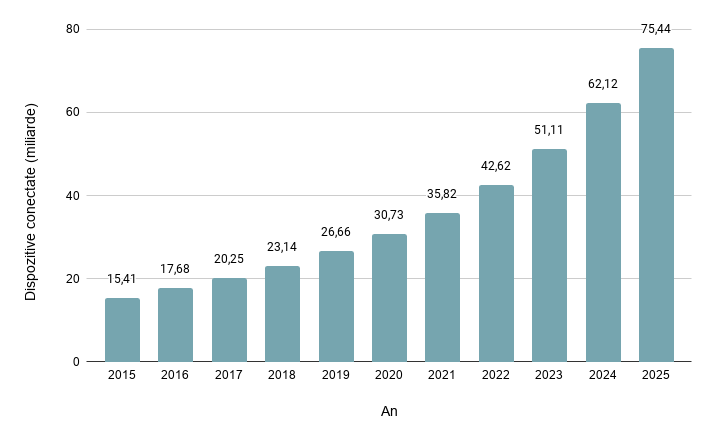
\includegraphics[width=\textwidth]{img/IoT_forecast.png}
\caption{Dispozitive IoT conectate la nivel mondial în perioada 2015-2025~\cite{statisca_Iot_forecast}\protect}
\label{fig:IoT_forescat}
\end{figure}

Dezvoltarea IoT și popularitatea acestora a condus la creșterea volumului de date în rețelele mobile, fapt care s-a lovit de limitările impuse de infrastructura companiilor telecom. Dezvoltarea optimă a dispozitivelor, folosirea celor mai inteligenți algoritmi sau controlul erorilor nu sunt suficiente pentru a asigura o bună calitate a experienței utilizatorilor. Pierderea pachetelor într-o rețea care este supraîncărcată sau timpii mari de răspuns reprezintă doar două dintre problemele care pot să apară ca urmare a limitărilor impuse de hardware-ul folosit de operatori. La nivel de rețea traficul este tratat la fel, indiferent de sursa acestuia, însă diversitatea lumii IoT are nevoie de mai mult de atât. Astfel de limitări au impact diferit asupra experienței pe care o resimt utilizatorii de streaming video în comparație cu efectele pe care le poate genera o funcționare defectuoasă a sistemelor cu care sunt dotate ambulanțele.

Pot fi identificate două planuri de acțiune, fie la nivelul tehnologiilor și hardware-ului deținut de companiile de telecom, fie la nivelul consumatorilor prin adaptarea software-ului care rulează pe dispozitive. Prima dintre ele nu este tocmai fezabilă din punct de vedere al costurilor pe care le-ar implica achiziționarea de noi echipamente, dar și reorganizarea infrastructurii și a arhitecturii deja existente. Astfel, atenția se îndreaptă asupra soluțiilor inteligente care se bazează pe algoritmi de offloading și rutarea traficului în funcție de caracteristicile acestuia.

Există limitări hardware și la nivelul utilizatorilor prin interfețele de care dispun (Wi-Fi, 3G, 4G, 5G, Bluetooth, etc.) sau a puterii de procesare. De asemenea, tipul de trafic generat poate varia de la streaming video, descărcare de software, trimiterea de fișiere, navigarea pe internet sau până la sistemele avansate de telemedicină cu care pot fi dotate ambulanțele, după cum se va detalia în capitolul următor.

Subiectul pe care îl tratează lucrarea are în vedere îmbunătățirea tehnicilor de offloading prin analizarea traficului, stabilirea unor metrici și măsurarea acestora în vederea alegerii interfeței pe care să fie trimis traficul, decongestionând astfel rețelele mobile și asigurând o bună funcționarea a dispozitivelor care se reflectă în experiența pe care o are utilizatorul.

\chapter{Motivație}
Marile companii de telecom întâmpină dificultăți odată cu creșterea cererii de date mobile, încercând să păstreze constantă viteza oferită. Conform Ericsson Mobility Report~\cite{ericsson_mobility_report}, apărut în 2019, se preconizează că traficul generat de telefoanele mobile va crește anual cu 27\% pe perioada 2019-2025. Aproximativ 63\% din totalul înregistrat în 2019 este reprezentat de trafic video și se prevede o creștere anuală de 30\% până în 2025, ajungând ca acesta să ocupe aproape trei sferturi din trafic~\cite{ericsson_mobility_report}. Traficul generat de aplicațiile mobile poate varia, Figura \ref{fig:tipuri_de_trafic}, iar o bună funcționare a acestora vine cu cerințe specifice.

\begin{figure}[th]
\centering
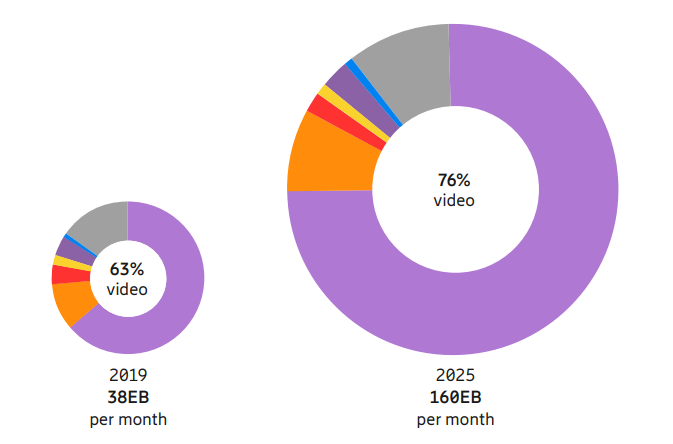
\includegraphics[width=\linewidth]{img/tipuri_de_trafic.png}
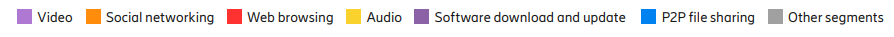
\includegraphics[width=\linewidth]{img/tipuri_de_trafic_legenda.png}
\caption{Trafic mobil pe categorii de aplicații (pe lună)~\cite{ericsson_mobility_report}\protect}
\label{fig:tipuri_de_trafic}
\end{figure}

Creșterea traficului video este datorată faptului că acesta a fost integrat în multe aplicații (Instagram, Facebook, etc.), pe lângă popularitatea de care se bucură din partea marilor furnizori de streaming video precum Netflix sau Amazon Prime Video. Variind de la o rețea la alta, rezoluția cea mai folosită pentru video este de 480p. Dezvoltarea de hardware inteligent și redarea de conținut video pe ecrane cât mai mici, la rezoluții cât mai bune duce la creșterea preferințelor pentru streaming-ul HD (720p) și Full HD (1080p)~\cite{ericsson_mobility_report}. Pentru ca utilizatorul să aibă parte de experiența dorită este nevoie de performanțe și din partea operatorilor de rețea.

În ceea ce privește traficului generat de rețele sociale este preconizată o creștere anuală cu 20\%, în următorii 6 ani. Cu toate acestea se va resimți o scădere a totalului cu un procent de 10\%, anul 2019, la 8\% în 2025, motivul fiind creșterea traficului video~\cite{ericsson_mobility_report}.

Dat fiind faptul că rețelele mobile fac din ce în ce mai greu față volumului de trafic pe care trebuie să-l gestioneze, în ultimii ani atenția s-a concentrat asupra măsurilor care pot fi luate la nivelul dispozitivelor generatoare de trafic. Prin aplicarea algoritmilor de offloading precum Greedy, Heuristic sau Random~\cite{offloading-jou}, performanța și experiența pe care le are utilizatorul sunt maximizate, având costuri minime. Luarea deciziilor de rutare și aplicarea optimă a algoritmilor de offloading se realizează prin analizarea unor metrici ce țin de tipul trafic, latență, lățime de bandă, calitatea semnalului sau durata de viață a bateriei.

Performanța unei rețele încărcate ce duce la pierderea de pachete poate fi considerată critică atunci când vine vorba de buna funcționare a sistemelor cu care sunt dotate mașinile de ambulanță. Cu toate că dezvoltatorii s-au concentrat pe controlul erorilor și o funcționare optimă a software-ului, aceștia nu au cum să compenseze lipsurile generate de pierderea pachetelor. 

Două cazuri de scenarii reale care necesită transmisiune multimedia de calitate sunt: un sistem de tratare de la distanță a bolnavilor aflați într-o ambulanță, și un sistem de monitorizare a terenurilor agricole în zone cu acoperire redusă.

În noiembrie 2019~\cite{use_case_ambulance}, în UK a avut loc un experiment în care un medic a asistat de la distanță un manechin aflat într-o ambulanță. Paramedicul aflat în mașină a purtat o mănușă parte dintr-un sistem conectat la rețeaua 5G, prin intermediul căreia medicul a putut, de la distanță, să efectueze scanarea cu ultrasunete a manechinului. De această dată ambulanța nu se afla în mișcare și medicul nu se afla la o distanță foarte mare de aceasta. În cazurile reale aceste două constante nu vor mai exista, iar calitatea transmisiunii va fi crucială pentru viața pacientului. Performanța rețelelor 4G, 5G, Wi-Fi sau latența minimă atunci când se face trecerea de la o celulă la altă, prin arii ce țin de operatori diferiți sunt elemente cheie în asigurarea sănătății pacientului. Este important ca datele colectate să fie transmise cât mai rapid și conexiunea să fie asigurată în permanență.

Primul caz real menționat anterior vizează limitările menționate mai sus prin dotarea a cinci ambulanțe cu un gateway inteligent. Acesta poate să monitorizeze comunicarea wireless pe mai multe canale, să ia decizii de rutare bazate pe Inteligență Artificială, fiind următorul pas către dezvoltarea tehnologiilor 6G care să facă față rețelelor eterogene și a menținerii conectivității între ariile de acoperire Wi-Fi sau 5G. Datele înregistrate trebuie să fie trimise către doctorii din spitale pentru diagnosticare și luarea măsurilor în condiții de urgență. Acest lucru depinde de performanța tehnologiilor de comunicare prezente în acea zonă (combinarea transmisiunii 3G, 4G, 5G, Wi-Fi, etc.), probleme ce țin de supraîncărcarea rețelei sau mecanisme de refacere a conexiunii care nu funcționează corespunzător.

Cel de al doilea caz se referă la colectarea datelor cu privire la gradul de poluare a aerului, în zone cu grad de acoperire redus. O dată cu încălzirea globală a crescut și numărul incendiilor ca urmare a gradului ridicat de poluare. Senzorii pot folosi tehnologii precum LoRa sau ZigBee care se dovedesc a fi mult mai eficiente în cazul unui dezastru natural. Nu calitatea comunicării este cea care contează acum, ci faptul că echipamentele de rețea să nu fie afectate și astfel se poată realiza comunicarea cu autoritățile. În acest caz, tehnologiile sunt limitate și trebuie să fie aleasă interfața corespunzătoare pentru ca datele să ajungă la server/cloud.

\chapter{Metode Existente}
Soluțiile actuale prezentate în literatura de specialitate precum și în articolele științifice oferă o imagine asupra nivelului curent de dezvoltare a tehnicilor de offloading care pot fi aplicate la nivelul telefoanelor mobile.

Congestia care apare la nivelul celulelor de comunicație nu poate fi rezolvată prin adăugare a și mai multe celule deoarece acest lucru ar duce la interferența semnalelor emise de acestea. O soluție constă în adăugarea de rețele Wi-Fi și tehnologii Long Term Evolution (LTE) care să poată prelua din traficul mobil destinat celulelor pentru a decongestiona rețeaua, lucru care se reflectă în calitatea serviciilor pe care le primește utilizatorul.

\section{Wi-Fi Offloading}
Frecvențele folosite de Wi-Fi (2.4GHz, 5GHz, 900MHz) nu interferează cu cele folosite de rețeaua 3G, iar acest lucru le-a permis operatorilor telecom, precum AT\&T, T-Mobile, Vodafone sau Orange, să îmbine cele două tehnologii peste tot în lume~\cite{offloading-jou}. Date fiind aceste modificări la nivelul infrastructurii, dezvoltatorii de aplicații software au profitat de oportunitățile oferite. \textbf{Line2 iPhone}~\cite{line2} este o aplicație care prin clonare software-ului telefonului poate să inițieze apeluri telefonice folosind rețeaua Wi-Fi. O altă aplicație, \textbf{iPassConnect}~\cite{ipass} le permite utilizatorilor să facă trecerea rapid de la 3G la Wi-Fi în funcție de zona de acoperire. De asemenea, \textbf{Balasubramanian et al.}~\cite{balasubramanian} își îndreaptă atenția asupra aplicațiilor a căror funcționare nu este influențată de întârzierea răspunsului. Sistemul pe care aceștia îl dezvoltă se numește \textbf{Wiffler} și are ca scop creșterea capacității rețelelor 3G prin redirecționare traficului pe Wi-Fi în funcție de gradul de încărcare al rețelei și a timpului de răspuns maxim acceptat de aplicație.
Cu toate acestea, Wi-Fi vine cu limitări în funcție de aria în care sunt amplasate routerele (de exemplu, zone cu acoperire redusă). Astfel, atenția se mută asupra dispozitivelor aflate în proximitate și cum pot acestea să preia din traficul destinat către celule sau Wi-Fi.

\section{Bluetooth Offloading}
Cele mai multe dintre smartphone-uri vin dotate atât cu Bluetooth cât și cu antene pentru Wi-Fi. Pentru a se realiza comunicarea și offloading-ul de trafic către dispozitivele aflate în imediata apropiere, trebuie ca aceste să își facă cunoscută prezența. În articolul~\cite{offloading-jou} s-au făcut o serie de experimente care au condus la faptul că este mult mai eficient ca descoperirea dispozitivelor să se facă folosind Bluetooth, iar transferul de date să fie realizat prin Wi-Fi. Smartphone-urile pot să păstreze în cache informații de care pot avea nevoie alte dispozitive aflate în imediata apropiere. Atunci când se dorește descărcarea unui fișier, traficul nu va mai trece prin rețeaua celulară, datele necesare fiind preluate din cache-ul dispozitivului descoperit prin Bluetooth. Folosind Wi-Fi, transferul de date de la un dispozitiv la altul poate varia de la 54Mbps (802.11g) până la 600Mbps (802.11n)~\cite{offloading-jou}.

Pe lângă viteza de transfer, un factor foarte important îl reprezintă consumul de baterie. Au fost realizate măsurători, pe un telefon Nokia N900, în ceea ce privește durata de viață a bateriei în încercarea de a descoperi la intervale de 1, 3, 10 sau 30 de secunde dispozitivele aflate în jur. Concluzia la care s-a ajuns constă în faptul că este consumată mai puțină baterie atunci când descoperirea se face prin Bluetooth, comparativ cu varianta în care se utilizează Wi-Fi.

\section{Metrici relevante în aplicarea algoritmilor de offloading}
Este cunoscut faptul că rețelele sunt din ce în ce mai eterogene, înglobând celule de comunicație, Wi-Fi, Femtocells sau tehnologii Long Term Evolution (LTE). O dată cu acestă diversitate apar și o serie de provocări precum interferența sau menținerea conexiunilor și trecerea traficului de la o tehnologie la alta. În articolul~\cite{traffic_steering} sunt realizate măsurători ce țin de puterea semnalului primit (RSS) de la punctele de acces Wi-Fi (AP), dar și de nivelul consumului de baterie. De asemenea, sunt colectate metrici precum lățimea de bandă disponibilă, consumul de baterie folosind tehnologiile 3GPP sau ANDSF pentru descoperirea tehnologiilor non 3GPP disponibile în apropiere. 
S-a observat faptul că durata de viață a bateriei este prelungită atunci când traficul este trimis către punctele de acces Wi-Fi care suportă un debit mai mare de date.

\chapter{Concluzii}
Găsirea de soluții pentru decongestionarea rețelelor este un subiect de actualitate, iar aplicarea metodelor de offloading este una dintre acestea. Analizarea metodelor deja existente precum și modul acestora de funcționare reprezintă punctul de plecare pentru rezolvarea provocărilor care apar odată cu creșterea numărului de smartphone-uri și dispozitive IoT.

În continuare va fi realizată analiza traficului de date în rețelele mobile. Stabilirea de metrici și colectarea acestora se va realiza folosind platforma MONROE\protect\footnotemark \footnotetext{\url{https://github.com/MONROE-PROJECT/UserManual/blob/master/user\_manual.pdf}}, amplasată în clădirea Precis din campusul Universității Politehnica București. Hardware-ul platformei facilitează realizarea de măsurători și experimente, punând la dispoziției multiple interfețe precum Wi-Fi, 4G, GPS, ZTE MF910 LTE Cat4
MiFis și suport pentru cartele SIM. Analiza metricilor colectate va contribui la dezvoltarea de soluții de offloading în rețelele mobile.

\bibliographystyle{plain}
\bibliography{bibliography}

\end{document}